% !TEX TS-program = pdflatex
% !TEX encoding = UTF-8 Unicode 

% This is a simple template for a LaTeX document using the "article" class.
% See "book", "report", "letter" for other types of document.

\documentclass[11pt]{article} % use larger type; default would be 10pt

\usepackage[utf8]{inputenc} % set input encoding (not needed with XeLaTeX)

%%% Examples of Article customizations
% These packages are optional, depending whether you want the features they provide.
% See the LaTeX Companion or other references for full information.

%%% PAGE DIMENSIONS
\usepackage{geometry} % to change the page dimensions
\geometry{a4paper} % or letterpaper (US) or a5paper or....
\geometry{margin=1in} % for example, change the margins to 2 inches all round
% \geometry{landscape} % set up the page for landscape
%   read geometry.pdf for detailed page layout information

\usepackage{graphicx} % support the \includegraphics command and options
\usepackage{floatrow}
\usepackage{multirow}
\usepackage{url}

\usepackage[svgnames]{xcolor}
\usepackage{listings}

\lstset{language=R,
    basicstyle=\small\ttfamily,
    stringstyle=\color{DarkGreen},
    otherkeywords={0,1,2,3,4,5,6,7,8,9},
    morekeywords={TRUE,FALSE},
    deletekeywords={data,frame,length,as,character},
    keywordstyle=\color{blue},
    commentstyle=\color{DarkGreen},
}


% \usepackage[parfill]{parskip} % Activate to begin paragraphs with an empty line rather than an indent

%%% PACKAGES
\usepackage{booktabs} % for much better looking tables
\usepackage{array} % for better arrays (eg matrices) in maths
\usepackage{paralist} % very flexible & customisable lists (eg. enumerate/itemize, etc.)
\usepackage{verbatim} % adds environment for commenting out blocks of text & for better verbatim
\usepackage{subfig} % make it possible to include more than one captioned figure/table in a single float
% These packages are all incorporated in the memoir class to one degree or another...

%%% HEADERS & FOOTERS
\usepackage{fancyhdr} % This should be set AFTER setting up the page geometry
\pagestyle{fancy} % options: empty , plain , fancy
\renewcommand{\headrulewidth}{0pt} % customise the layout...
\lhead{}\chead{}\rhead{}
\lfoot{}\cfoot{\thepage}\rfoot{}

%%% SECTION TITLE APPEARANCE
\usepackage{sectsty}
\allsectionsfont{\sffamily\mdseries\upshape} % (See the fntguide.pdf for font help)
% (This matches ConTeXt defaults)

%%% ToC (table of contents) APPEARANCE
\usepackage[nottoc,notlof,notlot]{tocbibind} % Put the bibliography in the ToC
\usepackage[titles,subfigure]{tocloft} % Alter the style of the Table of Contents
\renewcommand{\cftsecfont}{\rmfamily\mdseries\upshape}
\renewcommand{\cftsecpagefont}{\rmfamily\mdseries\upshape} % No bold!

%%% END Article customizations

%%% The "real" document content comes below...

\title{Introduction to Machine Learning Assessment}
\author{Michael Hoskin}
\date{} % Activate to display a given date or no date (if empty),
         % otherwise the current date is printed 

\begin{document}
\maketitle

\section{Introduction}


\subsection{Classification Problems}

Within machine learning, a classification problem is one where labelled training data is used to attempt to classify unlabelled test data. It falls under the remit of supervised learning -  i.e. the classifier is given target output values for the training set, rather than just attempting to cluster data into homogeneous groups. 

For training observations $X$, with labels $Y$, we try to find a function $f : x \rightarrow y$, so that for an unknown observation, $f(x)$ can predict with a high success rate the output $y$.

K-Nearest-Neighbours (KNN) is a simple but powerful classification algorithm. It is non-parametric, in that it makes no explicit assumptions about the form of $h$ and avoids the risk of attributing an incorrect distribution to the data. It is also instance-based, in that it doesn't create or learn a model, instead the only output of running a KNN on a data set is a an array of predicted values to compare with the data's actual values. As the algorithm must store the entire data set in memory, there is both a large memory cost, and a large processing cost as the entire data set must be iterated over for each observation. 

Within the KNN algorithm, K must be chosen in advance. A very small K provides a flexible fit, but removes knowledge of overall distributions of points. A higher K however is more resilient to outlying data points, and will have smoother boundaries. Odd values of K reduce the possibility of tied values. 


\subsection{Training and Test Data Sets}

For classification problems, data sets are usually split into two, or three, parts: a training set and a test set.

The model, or classifier, is initially trained using the training data, which contains both input data to pass to the classifier, and output values, labels or targets for the classifier to compare results with. Based on this result, model parameters can be adjusted. 

Finally, the test data is used once a final model has been created, to test classifier performance on an independent dataset. If a classifier can fit both the training data, and the test data, it can be considered relatively free of overfitting. 


\subsection{Introduction to MNIST}

The MNIST (Modified National Institute of Standards and Technology) database is database of handwritten digits, and consists of 70,000 images, pre-split into 60,000 training images, and 10,000 test images. An example digit can be found in Figure \ref{fig:mnist_example}.



\begin{figure}[htb!]
\floatbox[{\capbeside\thisfloatsetup{capbesideposition={right,center},capbesidewidth=9cm}}]{figure}[\FBwidth]
{\caption{Example MNIST image denoting the digit '5', refactored from 1x784 to 27x27.}\label{fig:mnist_example}}
{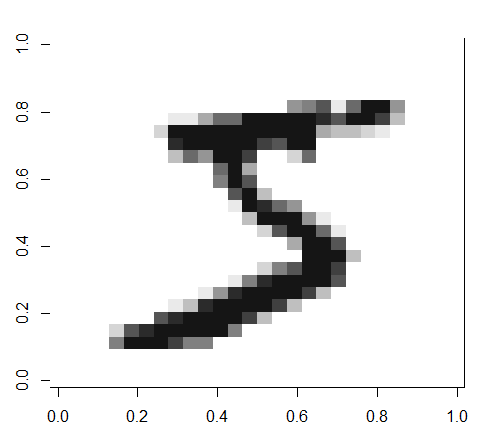
\includegraphics[width=0.15\textwidth]{mnist_example.png}}
\end{figure}

Each digit comes in the form of a 28x28 array of numbers between 0 and 255, representing a greyscale range. The digits have been size-normalised and centered. The data set as a whole originates from a much larger data set taken from NIST's (National Institute of Standards and Technology) Special Database 1 and Special Database 3. 30,000 images from each were selected to form the training set, and 5,000 of each selected to form the test set. SD-1 consists of digits written by high-school students, while SD-3 consists of digits written by employees of the US Census Bureau, and thus SD-3 digits are cleaner and easier to recognise than SD-1 digits. The split of digits into training and test was chosen to ensure that there is no overlap of author between the training and test sets - a random author will have digits in either the training data, or the test data, but not both. \cite{mnist-website}



\section{Dimensionality Reduction}

With the original MNIST data set, we can consider each observation to have 784 dimensions - one for each of the 28 x 28 pixel values, ranging from 0 to 255. If we can reduce this number to a number of key dimensions, we can avoid the 'curse of dimensionality', which arises when data is very sparse - as the number of dimensions increases, the amount of training data required to avoid overly sparse data increases exponentionally. It will also have the benefit of decreasing processing time of the classification algorithms used, as there are less dimensions to compute distances for. 

Principal Component Analysis (PCA) is one common method of unsupervised dimensionality reduction. Fundamentally it can be thought of of fitting an n-dimensional ellipsoid to a set of n dimensional data, where a long axis represents a feature with high variance. Principal components are new properties constructed from the original features, which can be used to summarise data; keeping only the first principal components retains large amounts of the key information for e.g. classifying  data. 

 Figure \ref{fig:pca_rotations_range} shows Eigenvalues relating to Principal Components 1 to 5, 101 to 105, and 601 to 605. While the first 5 can be recognised as numbers, the second set of 5 appear to be just noisy ovals, while the last set of 5 have very little meaningful data.  Figure \ref{fig:cumsum_pca} shows a cumulative plot revealing that - 87 PCs are enough to retain 90\% of the raw information. Diminishing returns occurs, so considering another 87 PCs increases this to only 95.8\%. 



\begin{figure}[htb!]
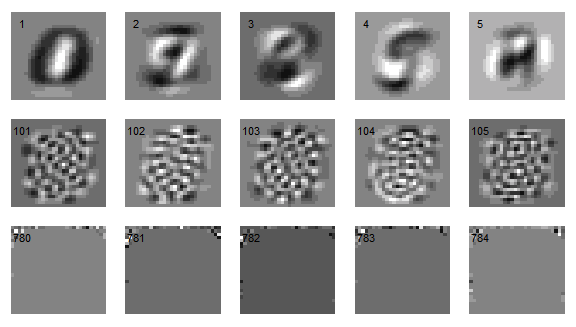
\includegraphics[width = 0.8\textwidth]{pca_rotations_wider_range.png}
\caption{Eigenvectors 1 to 5 (top), eigenvectors 101 to 105 (middle), and eigenvectors 601 to 605 (bottom). Original eigenvectors clearly represent a far greater amount of the original features.} 
\label{fig:pca_rotations_range}
\end{figure}

\begin{figure}[htb!]
\floatbox[{\capbeside\thisfloatsetup{capbesideposition={center,left},capbesidewidth=4cm}}]{figure}[\FBwidth]
{\caption{Cumulative amount of original variance kept as number of Principal Components (PCs) used increases. 87 PCs contain 90\% of the original data. Another 87 PCs increases this to 95.8\%.}\label{fig:cumsum_pca}}
{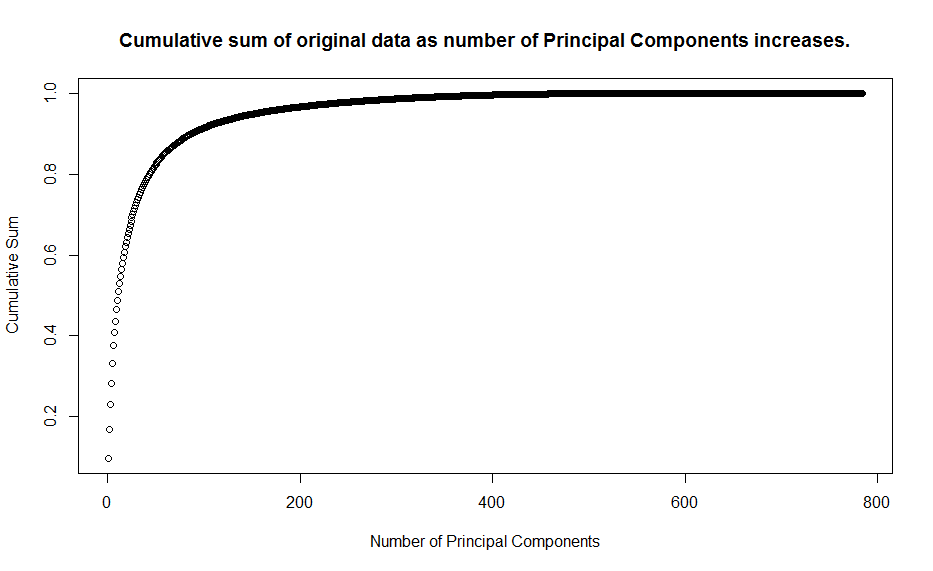
\includegraphics[width=0.8\textwidth]{cumulative_pca.png}}
\end{figure}

Applying PCA before running a KNN algorithm should filter out noise, by reducing features to new properties with high variance, and reduce processing time, by reducing the number of variables to consider from 784, to a more reasonable amount; as seen in Figure \ref{fig:cumsum_pca}, 87 PCs includes 90\% of the original features, while doubling the number of PCs only increases the amount of the original information retained by about 5\%.




\section{KNN}

\subsection{No preprocessing}

\subsubsection{First 10 Percent Training}

Initial classification attempts occurred with no attempts at pre-processing the data with dimensionality reduction, and instead just passed the first 6,000 training images, and the first 1,000 test images, into the knn function. The MNIST dataset tends to get noisier, and less clear as the index increases, so while it should be good at classifiying the early images, it should struggle with later ones. 





\subsubsection{Random 10 Percent Training}

By taking a random sample of the training data, we can train our KNN on a more representative sample of the data. Again, 10\% of the data is used, and the KNN is evaluated on a random 10\% of the test data. 



Here, the same training data is used to evaluate the entirety of the test data. 

\begin{figure}[htb!]
\floatbox[{\capbeside\thisfloatsetup{capbesideposition={center,right},capbesidewidth=5cm}}]{figure}[\FBwidth]
{\caption{Comparison of different KNN training samples. Red is training and testing on first 10\% of respective data sets. Green is training and testing on random 10\% of respective data sets. Blue is training on random 10\% and testing on all test data.}\label{fig:init_knn}}
{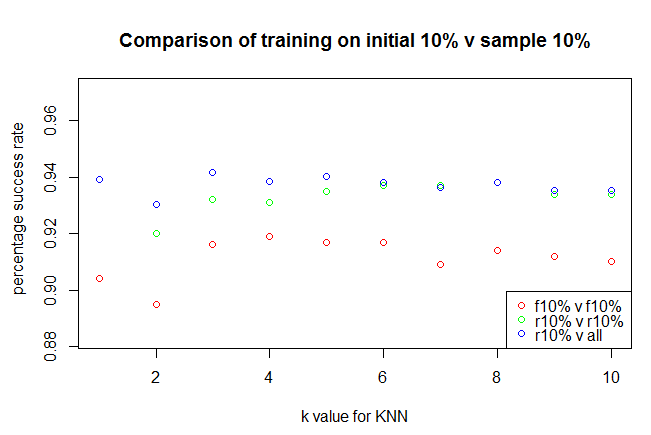
\includegraphics[width=0.6\textwidth]{10pc_training.png}}
\end{figure}



Figure \ref{fig:init_knn} (and the raw data table, Table \ref{rand-10-all-test} from Appendix \ref{sec:AppData}) shows that the random 10\% sample tested on all data the highest success rate was from setting K to $3$, and yielded a success rate of 0.9415 - failing on only about 1 in 20 images. This is about 2\% higher on average than just taking the first 10\% of the training data. 





\subsection{PCA}

After applying principal component analysis, the KNN algorithm was run again, varying the number of PCs from 2 to 50, and varying the ange of k values, from 1 to 17. Figure \ref{fig:pca_rkvar} shows the first three plots for varying k values, showing success rates against both the training dataset of 6000 random images, and the test dataset of all 10000 images.  50 PCs was chosen due to processing time; anything more 

As expected, the training rate is always higher than the test rate, and for k = 1, the training rate is unsuprisingly 1 for every number of PCs used. As the number of PCs used increases, the success rate of the test data increases, until a plateau is reached after about 20 - 25 PCs. The plateaus for different k values sit at around the 0.973 $\pm$ 0.001 mark, with a max value of 0.9759 at k = 3, nPCs = 34. As k increases, the training success rate decreases, while the test success rate stays fairly consistant. 

\begin{figure}[htb!]
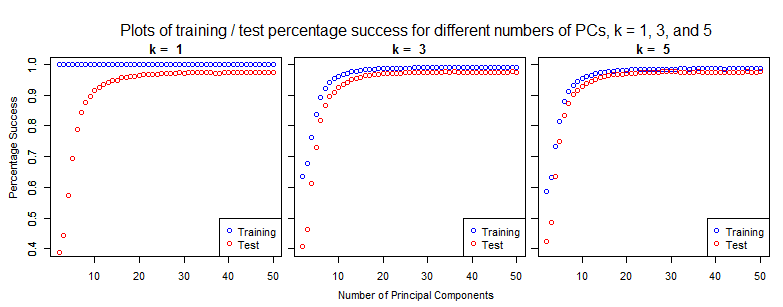
\includegraphics[width = 0.9\textwidth]{pca_kvar_traintest.png}
\caption{} 
\label{fig:pca_rkvar}
\end{figure}




\section{Neural Networks}

A different method of classification is using a neural network. These are inspired by biological neurons in the brain, and offer huge scope for efficient classification. Unlike KNNs, it is not instance based, and so a model is created which allows for evaluating test data repeatedly with a single model - this reduces the need to hold all data in memory while classifying; once the model is created, it can be reused repeatedly with minimal memory costs - evaluating the entire set of test data takes a neglible amount of time once the network has been trained.

The algorithm works by building a network of weighted connectors, generating output values and a cost function (error between output and calculated output), and then propagating back through the network to allow updating of weights between the connectors. This is iterated upon to reduce the cost function, until a minimum value is reached, or a maximum number of iterations is reached. 

First, the training data is normalised by dividing through by 255 (the maximum value of the greyscale array), and the labels are refactored into a 10 by x array of boolean flags for the benefit of the module.  The neural net is trained with a specific number of units in the hidden layer, for a defined number of iterations, before being used to predict output values with  a set of equally refactored test data. 

All neural networks were produced using the R function `nnet`' which only allows a single hidden layer between the input and output layers. The output neural net is an $x - y - 10$ network, where $x$ is the number of principal components - the number of input variables - and where $y$ is the size of the hidden layer, which varies from 30 to 60 throughout the following work. 

\subsection{Initial Tests}


Neural Nets were trained with all 60000 items of training data, and with other parameters varied as seen in Table \ref{nnet_parameters_init} within Appendix \ref{sec:AppData}. This process as a whole took approximately 24 hours (Windows 10, 12GB Ram, i5-4690k). Given the increase in correct classifications provided by preprocessing using PCA, all experiments were completed using the same PCA data as in the previous section.

The resulting data is summarised in the plots below. The results from the first plot, Figure \ref{fig:long_mean_nnet}, show an approximate 4\% increase in correct classification when increasing the number of iterations from 80 to 160, a hidden layer size of 40 correctly classifies more digits than ones of 30 or 50. The second plot, Figure \ref{fig:long_mean_pc_nnet}, shows that for a hidden layer size of 40, there is only a small benefit gained from increasing the number of Principal Components used. 

\begin{figure}[htb!]
\floatbox[{\capbeside\thisfloatsetup{capbesideposition={center,left},capbesidewidth=4cm}}]{figure}[\FBwidth]
{\caption{Plot of average success rate against number of iterations. Size of hidden layer is depicted by line colour. Success rate is averaged over all principal component values.}\label{fig:long_mean_nnet}}
{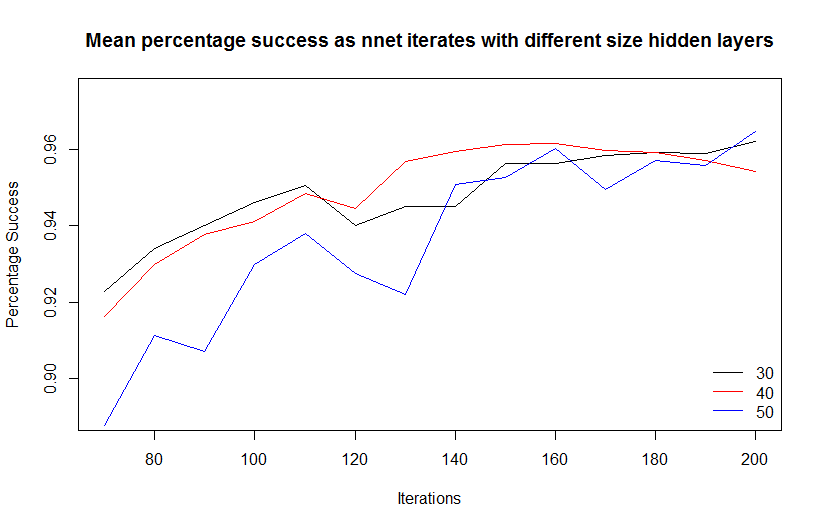
\includegraphics[width=0.7\textwidth]{long_mean_it.png}}
\end{figure}

\begin{figure}[htb!]
\floatbox[{\capbeside\thisfloatsetup{capbesideposition={center,right},capbesidewidth=4cm}}]{figure}[\FBwidth]
{\caption{Plot of average success rate against number of principal components used. Size of hidden layer is depicted by line colour. Success rate is averaged over all iterations from 110 onwards, reflecting the plateaued part of the percentage-iteration relationship.}\label{fig:long_mean_pc_nnet}}
{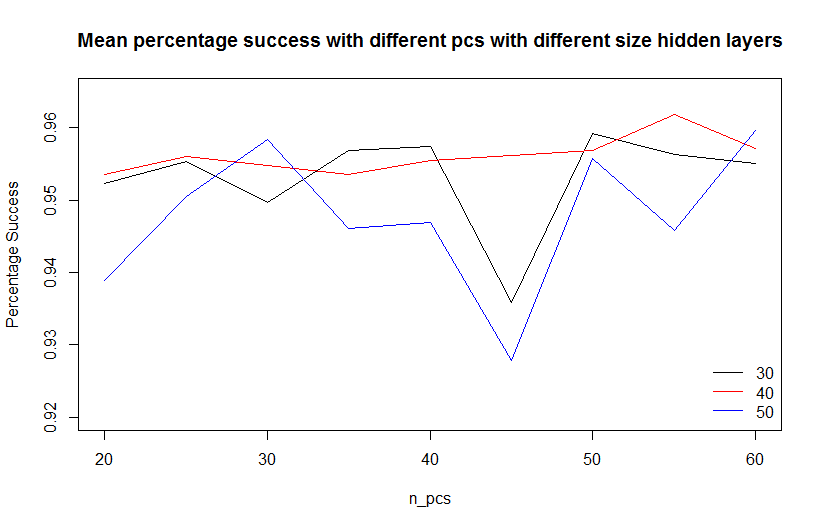
\includegraphics[width=0.7\textwidth]{long_mean_pcs_cutdown.png}}
\end{figure}

\subsection{Secondary Tests - Extended Iterations, Hidden Layer}

Given the Initial tests showed that the success rate increases with the number of iterations, secondary tests extending the number of iterations to 500 were completed. As seen in Table \ref{nnet_parameters_second} within Appendix \ref{sec:AppData}, neural nets were created with hidden layers from 40 to 60, with a smaller resolution of principal components to vary over, but going up to a higher value (70 rather than 60). Instead of iterating between 70 and 200 times, it iterates from 120 to 500. Again, this took approximately 24 hours - despite the greatly reduced number of variables to try, the higher iterations of nnet training unsuprisingly take a lot longer.

\begin{figure}[htb!]
\floatbox[{\capbeside\thisfloatsetup{capbesideposition={center,left},capbesidewidth=4cm}}]{figure}[\FBwidth]
{\caption{Plot of average success rate against number of iterations. Size of hidden layer is depicted by line colour. Success rate is averaged over all principal component values. }\label{fig:ext_mean_nnet}}
{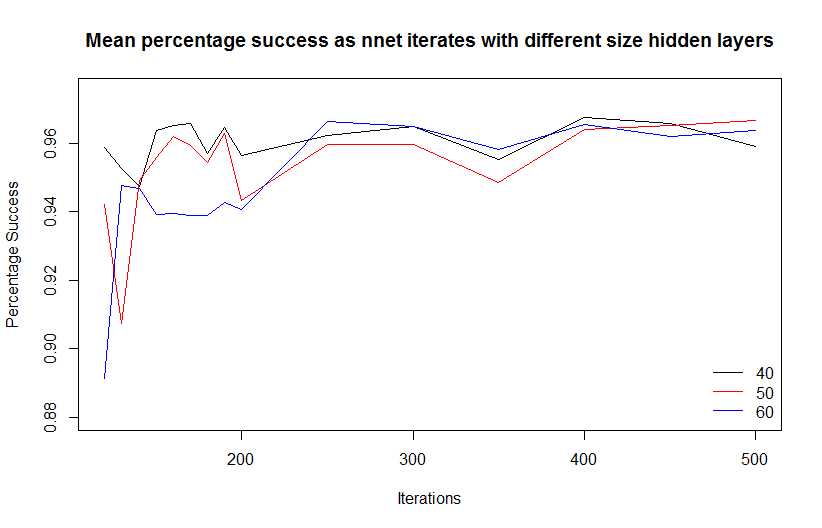
\includegraphics[width=0.7\textwidth]{nnet_extend_iter_mean.png}}
\end{figure}

\begin{figure}[htb!]
\floatbox[{\capbeside\thisfloatsetup{capbesideposition={center,right},capbesidewidth=4cm}}]{figure}[\FBwidth]
{\caption{Plot of average success rate against number of principal components used. Size of hidden layer is depicted by line colour. }\label{fig:ext_mean_pc_nnet}}
{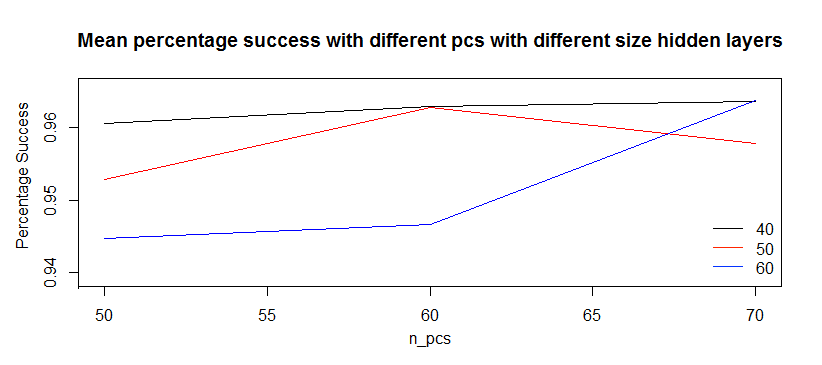
\includegraphics[width=0.7\textwidth]{nnet_mean_diff_pcs_extended_it2.png}}
\end{figure}

The highest success rate for 10,000 test images occurred with a 70-40-10 neural net, iterating 190 times, and yielded a 0.9692 success rate. 

\subsection{Tertiary Tests, Extended Iterations}

For the third set of tests, the size of the hidden layer was set to 40 for each neural net produced. Up to 3000 iterations were used, extending greatly the range used in previous trials. The number of principal components used varied from 50 to 150, again, reaching almost double the amount previously used.


\begin{figure}[htb!]
\floatbox[{\capbeside\thisfloatsetup{capbesideposition={center,left},capbesidewidth=4cm}}]{figure}[\FBwidth]
{\caption{Plot of success rate against number of iterations for different principal components used. }\label{fig:superext_nnet}}
{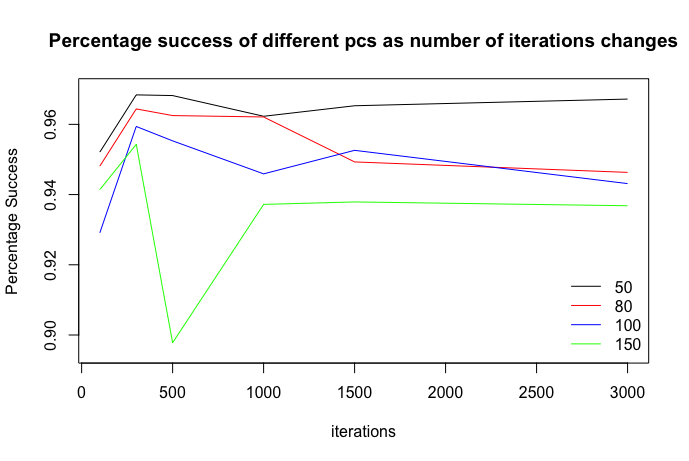
\includegraphics[width=0.7\textwidth]{nn_superext.png}}
\end{figure}

This data in Figure \ref{fig:superext_nnet} clearly shows increasing the number of principal components beyond 50 has a negative effect on the number of images correctly identified. It also shows that beyond a certain point - around 500 iterations - there is a general decrease in percentage success. 

The highest success rate for 10,000 test images occurred with a 50-40-10 neural net, iterating 300 times, and yielded a 0.9684 success rate.


\section{Analysis and Discussion}

\section{Conclusion}

\newpage
\begin{thebibliography}{9}



\bibitem{mnist-website} MNIST overview, \url{yann.lecun.com/exdb/mnist}, Accessed 2019-04-02
http://yann.lecun.com/exdb/mnist/
\end{thebibliography}

\newpage

\appendix
\label{appendix}
\section{Summary Data for KNN}
\label{sec:AppData}

\begin{table}[h]
\begin{center}
\begin{tabular}{l| c c c c c c c c c c}
 & 1 & 2 & 3 & 4 & 5 & 6 & 7 & 8 & 9 & 10\\
\hline
A & 0.904 & 0.895 & 0.916 & 0.919 & 0.917 & 0.917 & 0.909 & 0.914 & 0.912 & 0.910\\
B & 0.939 & 0.920 & 0.932 & 0.931 & 0.935 & 0.937 & 0.937 & 0.938 & 0.934 & 0.934\\
C & 0.9390 & 0.9303 & 0.9415 & 0.9383 & 0.9401 & 0.9381 & 0.9362 & 0.9380 & 0.9352 & 0.9354\\
\end{tabular}
\caption{Success rates for $k = 1:10$. A: trained on 6,000 random digits and tested on random 1,000 digits (Red in Fig \ref{fig:init_knn}). B: trained on 6,000 random digits and tested on random 1,000 digits (Green in Fig \ref{fig:init_knn}). C: trained on 6,000 random digits and tested on all 10,000 digits (Blue in Fig \ref{fig:init_knn}).}
\label{rand-10-all-test}
\end{center}
\end{table}

\section{PCA for KNN}
\label{sec:App_PCA}

\begin{figure}[htb!]
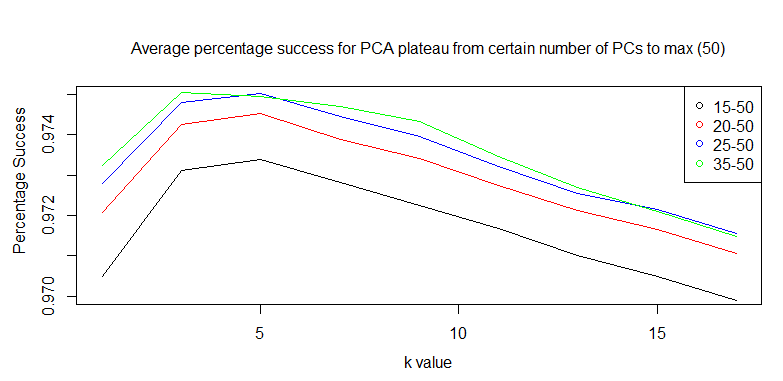
\includegraphics[width = 0.9\textwidth]{pca_knn_avplateau.png}
\caption{Shows the average percentage success across PCs from a s} 
\label{fig:pca_knn_avplateau}
\end{figure}

\section{Neural Network configurations}
\label{sec:AppNNetConfig}

\begin{table}[h!]
\begin{center}
\begin{tabular}{rl}
Parameter & Values \\
\hline
Hidden Layer Size & 30, 40, 50\\
Number of PCs & 20, 25, 30, 35, 40, 45, 50, 55, 60\\
Neural Net Iterations & 70, 80, 90, 100, 110, 120, 130,\\
& 140, 150, 160, 170, 180, 190, 200\\
\hline
\end{tabular}
\caption{Configuration values for initial Neural Network tests.}
\label{nnet_parameters_init}
\end{center}
\end{table}


\begin{table}[h!]
\begin{center}
\begin{tabular}{rl}
Parameter & Values \\
\hline
Hidden Layer Size & 40, 50, 60\\
Number of PCs & 50, 60, 70\\
Neural Net Iterations &  120, 130, 140, 150, 160, 170, 180, 190,\\
& 200, 250, 300, 350, 400, 450, 500\\
\hline
\end{tabular}
\caption{Configuration values for secondary Neural Network tests.}
\label{nnet_parameters_second}
\end{center}
\end{table}


\begin{table}[h!]
\begin{center}
\begin{tabular}{rl}
Parameter & Values \\
\hline
Hidden Layer Size & 40\\
Number of PCs & 50, 80, 100, 150\\
Neural Net Iterations & 100, 300, 500, 1000, 1500, 3000\\
\hline
\end{tabular}
\caption{Configuration values for tertiary Neural Network tests.}
\label{nnet_parameters_third}
\end{center}
\end{table}


\section{Source Code}

\subsection{Input Data}

Functions provided during course, `load\_mnist' function edited to take input paths. 
\begin{lstlisting}

# Load the MNIST digit recognition dataset into R
# http://yann.lecun.com/exdb/mnist/
# assume you have all 4 files and gunzip'd them
# creates train$n, train$x, train$y  and test$n, test$x, test$y
# e.g. train$x is a 60000 x 784 matrix, each row is one digit (28x28)
# call:  show_digit(train$x[5,])   to see a digit.
# brendan o'connor - gist.github.com/39760 - anyall.org
load_mnist <- function(train.path = 'data/train-images.idx3-ubyte',
                       test.path = 'data/t10k-images.idx3-ubyte',
                       train.labels.path = 'data/train-labels.idx1-ubyte',
                       test.labels.path = 'data/t10k-labels.idx1-ubyte') {
  load_image_file <- function(filename) {
    ret = list()
    f = file(filename,'rb')
    readBin(f,'integer',n=1,size=4,endian='big')
    ret$n = readBin(f,'integer',n=1,size=4,endian='big')
    nrow = readBin(f,'integer',n=1,size=4,endian='big')
    ncol = readBin(f,'integer',n=1,size=4,endian='big')
    x = readBin(f,'integer',n=ret$n*nrow*ncol,size=1,signed=F)
    ret$x = matrix(x, ncol=nrow*ncol, byrow=T)
    close(f)
    ret
  }
  load_label_file <- function(filename) {
    f = file(filename,'rb')
    readBin(f,'integer',n=1,size=4,endian='big')
    n = readBin(f,'integer',n=1,size=4,endian='big')
    y = readBin(f,'integer',n=n,size=1,signed=F)
    close(f)
    y
  }
  train <<- load_image_file(train.path)
  test <<- load_image_file(test.path)
  
  train$y <<- load_label_file(train.labels.path)
  test$y <<- load_label_file(test.labels.path)  
}

show_digit <- function(arr784, col=gray(12:1/12), ...) {
  image(matrix(arr784, nrow=28)[,28:1], col=col, ...)
}

\end{lstlisting}

\end{document}
